% =========================================================================== %
% Yes. This is a document.

\documentclass[
	english,
	aspectratio=169,
	table
]{beamer}

% =========================================================================== %
% Theme
\usepackage{scrlfile}
	\ReplacePackage{beamerthemeSHUR}{./sty/beamerthemeSHUR}
	\ReplacePackage{beamerinnerthemefancy}{./sty/beamerinnerthemefancy}
	\ReplacePackage{beamerouterthemedecolines}{./sty/beamerouterthemedecolines}
	\ReplacePackage{beamercolorthemechameleon}{./sty/beamercolorthemechameleon}

\usetheme[
	pageofpages=/,
	bullet=circle,
	titleline=true,
	alternativetitlepage=true,
	watermark="",
	watermarkheight=0px,
	watermarkheightmult=0
	]
{SHUR}

% =========================================================================== %
% the usual stuff

\usepackage[utf8]{inputenc}
\usepackage[T1]{fontenc}
\usepackage{babel}
\usepackage{lmodern}
\usepackage{microtype}
\usepackage{csquotes}
\usepackage{xspace}

\usepackage{tabularx}
\usepackage{booktabs}
\usepackage{multirow}

\usepackage{color, colortbl}
\usepackage{xcolor}
	\definecolor{tabhighlight}{RGB}{230,240,255}

\usepackage{tabto}

\usepackage{minted}
	\usemintedstyle{friendly}

\usepackage{tikz}
	\usetikzlibrary{positioning}
	\usetikzlibrary{matrix}
	\usetikzlibrary{shapes.geometric}
	\usetikzlibrary{backgrounds}
	\usetikzlibrary{calc}
	\usetikzlibrary{decorations.pathreplacing}
	\tikzstyle{every picture}+=[remember picture] 
\usepackage{adjustbox}

\usepackage[most]{tcolorbox}
	\tcbsetforeverylayer
		{colback=cyan!10!white,
		 colframe=cyan!75!black,
		 arc=0pt,
		 outer arc=0pt,
		 parbox=false
		}
	\newtcolorbox{codebox}[1][Code]
		{colback=black!5!white,
		 colframe=blue!40!black,
		 title=#1,
		 leftupper=6mm
		}
	\newtcolorbox{cmdbox}[1][Kommandozeilen-Befehl]
		{colback=black,
		 coltext=white,
		 fontupper=\ttfamily ,
		 colframe=blue!40!black,
		 title=#1,
		 outer arc=0pt
		}
	\newtcolorbox{warnbox}[1][Beachte]
		{colback=black!5!white,
		 colframe=red!40!black,
		 title=#1
		}
	\newtcolorbox{hintbox}[1][Tipp]
		{colback=black!5!white,
		 colframe=green!40!black,
		 title=#1
		}
	\newenvironment{itembox}
		{\begin{tcolorbox}\begin{itemize}}%
		{\end{itemize}\end{tcolorbox}}
	\newtcolorbox{doublebox}[1][.3]
		{righthand width=#1\linewidth,
		 sidebyside,
		 sidebyside gap=6mm,
		 sidebyside align=center,
		 lower separated=false}
	
%==============================================================================%
% GLOBAL MACROS

\newcommand*{\eg}{e.\,g. }
\newcommand*{\ie}{i.\,e. }

\newcommand{\Thus}{\ensuremath{\Rightarrow}\xspace}
\newcommand{\thus}{\ensuremath{\rightarrow}\xspace}

\newcommand*{\tabcrlf}{\\ \midrule}			% actually still allows for optional argument

\newcommand*{\inPy}[1]{\mintinline{python}{#1}}

% =========================================================================== %

\author{Stefan Hartinger}
\title{Programming in Python}
\subtitle{Part 6: Functions}
\institute{University Regensburg, Department of Theoretical Physics}
\date{Winter Term 2021/22}

% =========================================================================== %

\begin{document}
% =========================================================================== %

\begin{frame}[t,plain]
\titlepage
\end{frame}

% =========================================================================== %

\begin{frame}{Recap}
%
\begin{itemize}
\item \inPy{while}-loops
	\begin{itemize}
	\item Repeat code as long as (\emph{while}) a condition is satisfied
	\end{itemize}
\item \inPy{break} and \inPy{continue}
	\begin{itemize}
	\item Stop looping early (\inPy{break}) or skip part of the loop body (\inPy{continue})
	\end{itemize}
\item \inPy{else} with \inPy{for} and \inPy{while}
	\begin{itemize}
	\item Execute code only when end of loop is reached (\inPy{for}) ...
	\item ... or when exited via \inPy{break} (\inPy{while})
	\end{itemize}
\end{itemize}
%
\begin{center}
	\emph{Any Questions?}
\end{center}
%
\end{frame}

% =========================================================================== %

\begin{frame}[fragile]{Chapter 6}
%
\begin{itemize}
\item Functions
\item By-Value- and By-Reference-Parameters
\item Scopes
\end{itemize}
%
\end{frame}

% =========================================================================== %

\begin{frame}[fragile]
%
\begin{columns}[T]
\column{.5\linewidth}
\begin{Large}
{Functions}
\vspace{6pt}
\end{Large}
\begin{itemize}
\item Idea: Combine multiple, recurring steps into a single command
\item Can be parametrised (Example: Output of text in a box)
\item Can return a result (\Thus \emph{function} in its mathematical sense)
\item \inPy{return}: exit function, return to where it was called
\item \inPy{return result}: same as above, plus: \enquote{report} a result
\item Without \inPy{return}: jump-back automatically after last command
\item Implicit return value \inPy{None}
\end{itemize}
%
\column{.5\linewidth}
\begin{codebox}[Syntax: Definition of Functions]
\begin{minted}[fontsize=\scriptsize]{python}
def functionName (parameters) :
    statements
    return result
\end{minted}
\end{codebox}
%
\begin{codebox}[Syntax: Calling a Function]
\begin{minted}[fontsize=\scriptsize]{python}
functionName(parameters)
variable = functionName(parameterlist)
\end{minted}
\end{codebox}
%
\begin{hintbox}[Order of Code]
Functions have to be defined \emph{before} they are called for the first time.
\end{hintbox}
\end{columns}
%
\end{frame}

% =========================================================================== %

\begin{frame}[fragile]
%
\begin{codebox}[Example: Simple Functions]
\begin{minted}[linenos, fontsize=\scriptsize]{python3}
def printHeadline() :
    print("# ========================================================= #")
    print("#                        H e a d l i n e                    #")
    print("# ========================================================= #")
    return
    print("this code will never be executed")

def polynomial(x) :
    return x**2 - 5*x + 3

def total(a, b)
    return a + b
    
printHeadline()
print( polynomial(5) )                    # Output: 3
print( total("some", " text") )           # Output: some text
\end{minted}
\end{codebox}
%
\end{frame}

% =========================================================================== %

\begin{frame}{Local Variables and Scopes}
%
\begin{itemize}
\item Desire: Function call should have no side effects
\item But: Functions may need to use auxillary variables
	\begin{itemize}
	\item Values stay in memory \thus side effect
	\item May overwrite other values if variable name already in use \thus side effect
	\end{itemize}
\item Solution: Functions have their own variables
	\begin{itemize}
	\item Function as a closed box, separate from rest of the code
	\item Not just jumping around, but starting an independent process
	\end{itemize}
\item Term \emph{Scope}
	\begin{itemize}
	\item Idea of \enquote{lifetime of a variable}
	\item Symbol only exists in a given range of code
	\item Variable is deleted when exiting the function
	\item May temporarily overwrite another symbol
	\end{itemize}
\end{itemize}
%
\end{frame}

% =========================================================================== %

\begin{frame}[fragile]
%
\begin{codebox}[Example: Scopes]
\begin{minted}[linenos, fontsize=\scriptsize]{python3}
def func() :
    x = 5
    y = 5
    print(x, y)           # Output: 5 5

x = 7
print(x)                  # Output: 7
func()
print(x)                  # Output: 7
# print(y)                # Error: y not defined in this scope!
\end{minted}
\end{codebox}
%
\end{frame}

% =========================================================================== %

\begin{frame}[fragile]{Parameters (aka Arguments)}
%
\begin{itemize}
\item Parameters: local variables!
\item Initialized with a \emph{copy} of the value in the call parameter list
\item Idea: \enquote{Send information into the function}
\end{itemize}
%
\vspace{5pt}
\begin{tcbraster}[raster columns=2,
                  raster equal height,
                  nobeforeafter,
                  raster column skip=0.5cm]
\begin{codebox}[Example: Evolution of Values]
\begin{minted}[fontsize=\scriptsize, linenos]{python}
def func(x, y) :
   print(x, y)
   x, y = 5, 5
   print(x, y)

x = 3
func(x, x + 5)
print(x)   
\end{minted}
\end{codebox}
%
\begin{tcolorbox}[title=Evolution of Values]
\scriptsize
\begin{center}
\begin{tabular}{l|ccc}
Line & $x_{main}$ & $x_{func}$ & $y_{func}$ \tabcrlf
6 & 3 & -- & -- \\
2 & 3 &  3 &  8 \\
3 & 3 &  5 &  5 \\
4 & 3 &  5 &  5 \\
8 & 3 & -- & --
\end{tabular}
\end{center}
\end{tcolorbox}
\end{tcbraster}
%
\end{frame}

% =========================================================================== %

\begin{frame}[fragile]
%
\vspace{-5pt}
\begin{codebox}[Example: Exponential as a Function]
\begin{minted}[linenos, fontsize=\scriptsize]{python}
def expFunction(x0) :
    x           = 1.0
    denominator = 1.0
    result      = 1.0
    iterations  = 10
    for k in range(1, iterations) :
        x            *= x0
        denominator  *= k
        result += x / denominator
    return result

result = expFunction(1.0)                   # Call function, store result in variable
print(f"Euler's Number is {result}")
print(f"e³ = {expFunction(3.0)}")           # Forward result to another function
\end{minted}
\end{codebox}

\begin{cmdbox}[Output: Exponential as a Function]
\begin{minted}[fontsize=\scriptsize]{text}
Euler's Number is 2.7182815255731922
e³ = 20.063392857142855
\end{minted}
\end{cmdbox}
%
\end{frame}

% =========================================================================== %

\begin{frame}[fragile]
%
\vspace{-7pt}
\begin{codebox}[Example: Function \enquote{without} Return Value]
\begin{minted}[linenos, fontsize=\scriptsize]{python}
import math

def printBoxed(text, boxSize) :
    lenText     = len(text)
    countSpaces = boxSize - lenText - 2        # 2 spaces for |borders|
    spacesLeft  = math.floor(countSpaces / 2)  # round down
    spacesRight = math.ceil (countSpaces / 2)  # round up
    print("+" +               (boxSize - 2) * "-"           + "+")
    print("|" + spacesLeft * " " + text + spacesRight * " " + "|")
    print("+" +               (boxSize - 2) * "-"           + "+")

reVal = printBoxed("Don't forget to be awesome!", 60)
print("The function returned:" , reVal)
\end{minted}
\end{codebox}

\vspace{-12pt}
\begin{cmdbox}[Output: Function \enquote{without} Return Value]
\begin{minted}[fontsize=\scriptsize]{text}
+----------------------------------------------------------+
|               Don't forget to be awesome!                |
+----------------------------------------------------------+
The function returned: None
\end{minted}
\end{cmdbox}
%
\end{frame}

% =========================================================================== %

\begin{frame}[fragile]{By-Value und By-Reference-Parameter}
%
\begin{itemize}
\item IT: World: two standards for functions: pass by value and by reference
\item By value: pure working copy.
\item By reference: where to find the information
\item Python: \emph{working copy of reference}
\item (Im)mutability and memory location affect outcome
\end{itemize}
%
\begin{tcbraster}[raster columns=2,
                  raster equal height,
                  nobeforeafter,
                  raster column skip=0.5cm]
\begin{codebox}[Example: Passing Mutables]
\begin{minted}[fontsize=\scriptsize, linenos]{python}
def foobar(data) :
    data.append(1)
    data = data + [2]
    print("in foobar: data =", data)
data = []
foobar(data)
print("on module level: data =", data)
\end{minted}
\end{codebox}
%
\begin{cmdbox}[Output: Passing Mutables]
\begin{minted}[fontsize=\scriptsize]{text}
in foobar: data = [1, 2]
on module level: data = [1]
\end{minted}
\end{cmdbox}
\end{tcbraster}
%
\end{frame}

% =========================================================================== %

\begin{frame}[fragile]
%
\begin{tcolorbox}[title=Memory Model]
\begin{center}
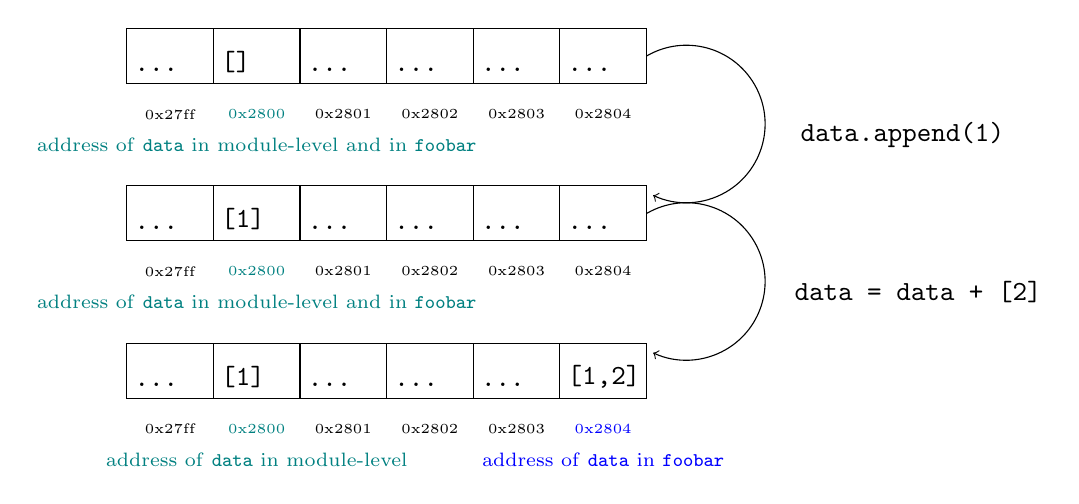
\begin{tikzpicture}
  [ 
    cell/.style={
      text width=9mm,
      text height=4mm,
      draw=black,
      inner sep=1mm,
      minimum height=7mm
    },
    ld/.style={draw=blue,shorten >=2pt,->}
  ]
  \node (a1) at (0.0,4) [cell] {\ttfamily ...};
  \node (a2) at (1.1,4) [cell] {\ttfamily  []};
  \node (a3) at (2.2,4) [cell] {\ttfamily ...};
  \node (a4) at (3.3,4) [cell] {\ttfamily ...};
  \node (a5) at (4.4,4) [cell] {\ttfamily ...};
  \node (a6) at (5.5,4) [cell] {\ttfamily ...};

  \node (b1) at (0.0,2) [cell] {\ttfamily ...};
  \node (b2) at (1.1,2) [cell] {\ttfamily [1]};
  \node (b3) at (2.2,2) [cell] {\ttfamily ...};
  \node (b4) at (3.3,2) [cell] {\ttfamily ...};
  \node (b5) at (4.4,2) [cell] {\ttfamily ...};
  \node (b6) at (5.5,2) [cell] {\ttfamily ...};

  \node (c1) at (0.0,0) [cell] {\ttfamily ...};
  \node (c2) at (1.1,0) [cell] {\ttfamily [1]};
  \node (c3) at (2.2,0) [cell] {\ttfamily ...};
  \node (c4) at (3.3,0) [cell] {\ttfamily ...};
  \node (c5) at (4.4,0) [cell] {\ttfamily ...};
  \node (c6) at (5.5,0) [cell] {\ttfamily [1,2]};
  
  \node (A1) [below=2mm of a1]             {\tiny 0x27ff};
  \node (A2) [below=2mm of a2, color=teal] {\tiny 0x2800};
  \node (A3) [below=2mm of a3]             {\tiny 0x2801};
  \node (A4) [below=2mm of a4]             {\tiny 0x2802};
  \node (A5) [below=2mm of a5]             {\tiny 0x2803};
  \node (A6) [below=2mm of a6]             {\tiny 0x2804};
  
  \node (B1) [below=2mm of b1]             {\tiny 0x27ff};
  \node (B2) [below=2mm of b2, color=teal] {\tiny 0x2800};
  \node (B3) [below=2mm of b3]             {\tiny 0x2801};
  \node (B4) [below=2mm of b4]             {\tiny 0x2802};
  \node (B5) [below=2mm of b5]             {\tiny 0x2803};
  \node (B6) [below=2mm of b6]             {\tiny 0x2804};
  
  \node (C1) [below=2mm of c1]             {\tiny 0x27ff};
  \node (C2) [below=2mm of c2, color=teal] {\tiny 0x2800};
  \node (C3) [below=2mm of c3]             {\tiny 0x2801};
  \node (C4) [below=2mm of c4]             {\tiny 0x2802};
  \node (C5) [below=2mm of c5]             {\tiny 0x2803};
  \node (C6) [below=2mm of c6, color=blue] {\tiny 0x2804};



  \node (main1) [below=0mm of A2, color=teal] {\scriptsize address of \texttt{data} in module-level and in \texttt{foobar}};
  \node (main2) [below=0mm of B2, color=teal] {\scriptsize address of \texttt{data} in module-level and in \texttt{foobar}};
  \node (main3) [below=0mm of C2, color=teal] {\scriptsize address of \texttt{data} in module-level};
  \node (func)  [below=0mm of C6, color=blue] {\scriptsize address of \texttt{data} in \texttt{foobar}};
  
  \draw [->] (a6.east)arc(120:-115:1.0);		%start angle: stop angle : radius  
  \node (step1) at (9.3,3) {\texttt{data.append(1)}};
  \draw [->] (b6.east)arc(120:-115:1.0);
  \node (step1) at (9.5,1) {\texttt{data = data + [2]}};
\end{tikzpicture}
\end{center}
\end{tcolorbox}
%
\end{frame}

% =========================================================================== %\\

\begin{frame}[fragile]
%
\begin{tcolorbox}[title=Memory Model: \texttt{int}s]
What does \inPy{x = 1337} look like internally?
\vspace{20pt}
\begin{center}
\begin{tikzpicture}
  [ 
    cell/.style={text width=8mm,
      text height=4mm, draw=black, inner sep=1mm},
    ld/.style={draw=blue,shorten >=2pt,->}
  ]
  
  \node  (invisible) at (-2, -0.25) {};
  \node  (a0) at ( 0,0) [cell] {\ttfamily  ...};
  \node  (a1) at ( 1,0) [cell] {\ttfamily @int};
  \node  (a2) at ( 2,0) [cell] {\ttfamily @dat};
  \node  (a3) at ( 3,0) [cell] {\ttfamily  8  };
  \node  (a4) at ( 4,0) [cell] {\ttfamily  ...};
  \node  (a5) at ( 5,0) [cell] {\ttfamily  ...};
  \node  (a6) at ( 6,0) [cell] {\ttfamily 1337};
  \node  (a7) at ( 7,0) [cell] {\ttfamily  ...};
  
  \node (b0) [above=1mm of a0] {\tiny 0xEFF8};
  \node (b1) [above=1mm of a1, color=teal] {\tiny 0xF000};
  \node (b2) [above=1mm of a2] {\tiny 0xF008};
  \node (b3) [above=1mm of a3] {\tiny 0xF010};
  \node (b4) [above=1mm of a4] {\tiny 0xF018};
  \node (b5) [above=1mm of a5] {\tiny 0xF020};
  \node (b6) [above=1mm of a6] {\tiny 0xF028};
  \node (b7) [above=1mm of a7] {\tiny 0xF030};
  
  \draw [decorate, decoration={brace,amplitude=7pt}, xshift=-0pt, yshift=0pt]
  		(+0.5, 1.0) -- ( 3.5, 1.0) node (x) [midway, yshift=+0.5cm] 
		(braceDescriptor) {Descriptor of \texttt{x}};
	
  \draw [decorate, decoration={brace,amplitude=7pt}, xshift=-0pt, yshift=0pt]
  		( 5.5, 1.0) -- ( 6.5, 1.0) node (y) [midway, yshift=+0.5cm] 
		(braceContent) {Use data of \texttt{x}};

	\draw [->, bend right=20]
		(a2.south) to node 
		[below] {cell content: 0xF028} 
		(a6.south);
			
	\draw [->, bend left=20]
		(a1.south) to node 
		[below] {cell content: ID of class \inPy{int}} 
		(invisible.south);
		
\end{tikzpicture}
\end{center}

\vspace{20pt}
Internally, \texttt{x} is only the \emph{address of the descriptor}, \ie the value \texttt{0xF000}.\\
Any access to the \emph{value of \texttt{x}} goes through a series of interpreteation steps!
\end{tcolorbox}
%
\end{frame}

% =========================================================================== %\\

\begin{frame}[fragile]
%
\begin{tcolorbox}[title=Memory Model: \texttt{list}s]
What does \inPy{lst = [x, 666]} look like internally?
\vspace{10pt}
\begin{center}
\begin{tikzpicture}
  [ 
    cell/.style={text width=8mm,
      text height=4mm, draw=black, inner sep=1mm},
    ld/.style={draw=blue,shorten >=2pt,->}
  ]
  
  \node  (invisible) at (-2, -0.25) {};
  \node  (a0) at ( 0,0) [cell] {\ttfamily  ...};
  \node  (a1) at ( 1,0) [cell] {\ttfamily @lst};
  \node  (a2) at ( 2,0) [cell] {\ttfamily @dat};
  \node  (a3) at ( 3,0) [cell] {\ttfamily  16 };
  \node  (a4) at ( 4,0) [cell] {\ttfamily  ...};
  \node  (a5) at ( 5,0) [cell] {\ttfamily  ...};
  \node  (a6) at ( 6,0) [cell] {\ttfamily @x  };
  \node  (a7) at ( 7,0) [cell] {\ttfamily @666};
  \node  (a8) at ( 8,0) [cell] {\ttfamily  ...};
  
  \node (b0) [above=1mm of a0] {\tiny 0xF030};
  \node (b1) [above=1mm of a1, color=teal] {\tiny 0xF000};
  \node (b2) [above=1mm of a2] {\tiny 0xF038};
  \node (b3) [above=1mm of a3] {\tiny 0xF040};
  \node (b4) [above=1mm of a4] {\tiny 0xF048};
  \node (b5) [above=1mm of a5] {\tiny 0xF050};
  \node (b6) [above=1mm of a6] {\tiny 0xF058};
  \node (b7) [above=1mm of a7] {\tiny 0xF060};
  \node (b8) [above=1mm of a8] {\tiny 0xF068};
  
  \draw [decorate, decoration={brace,amplitude=7pt}, xshift=-0pt, yshift=0pt]
  		(+0.5, 1.0) -- ( 3.5, 1.0) node (x) [midway, yshift=+0.5cm] 
		(braceDescriptor) {Descriptor of \texttt{lst}};
	
  \draw [decorate, decoration={brace,amplitude=7pt}, xshift=-0pt, yshift=0pt]
  		( 5.5, 1.0) -- ( 7.5, 1.0) node (y) [midway, yshift=+0.5cm] 
		(braceContent) {Use data of \texttt{lst}};

	\draw [->, bend right=20]
		(a2.south) to node 
		[below] {cell content: 0xF058} 
		(a6.south);
			
	\draw [->, bend left=20]
		(a1.south) to node 
		[below] {cell content: ID of class \inPy{list}}
		(invisible.south);
	
	\node (t6) at (6.8,-1.5) {\texttt{0xF028}};
	\node (t7) at (8.5,-1.5) {\texttt{0xF430}};
	
	\draw [->, bend right=15] (a6.south) to node [below] {} (t6.north);
	\draw [->, bend right=15] (a7.south) to node [below] {} (t7.north);
\end{tikzpicture}
\end{center}

\vspace{10pt}
The content of lists is actually only a series of addresses: each address references an object descriptor, even for literal constants! For constants, like \inPy{666} a new object descriptor is constructed \emph{somewhere}. They have no (exposed) symbol.
\end{tcolorbox}
%
\end{frame}

% =========================================================================== %

\begin{frame}[fragile]
%
\begin{codebox}[Example: Passing Immutables]
\begin{minted}[linenos, fontsize=\scriptsize]{python}
def foobar(data) :
    data = 2           # immutable object is reconstructed somewhere else
    print("in foobar: data =", data)

data = 1
foobar(data)
print("on module level: data =", data)
\end{minted}
\end{codebox}

\begin{cmdbox}[Output: Passing Immutables]
\begin{minted}[fontsize=\scriptsize]{text}
in foobar: data = 2
on module level: data = 1
\end{minted}
\end{cmdbox}
%
\end{frame}

% =========================================================================== %

\begin{frame}{Nonlocal Variables}
%
\begin{itemize}
\item Variables in a function are not visible in another function or on module level
\item But: variables on module level are visible in functions!
\item Also holds for nested scopes (nested functions)
\item \enquote{Can't see into a scope, but out of a scope}
\item[\Thus] Variables not local to their function do exist
\item Type of first access in a function defines behaviour
	\begin{itemize}
	\item Read access: nonlocal variable -- symbol stands for the variable in the higher scope
	\item Write access: local variable -- symbol is a new object
	\item Forbidden: operations that would change the memory address
	\item[\Thus] No mixed read/write access!
	\end{itemize}
\end{itemize}
%
\end{frame}

% =========================================================================== %

\begin{frame}[fragile]
%
\begin{tcbraster}[raster columns=2,
                  raster equal height,
                  nobeforeafter,
                  raster column skip=0.5cm]
\begin{codebox}[Example: Nonlocal Variables (1)]
\begin{minted}[fontsize=\scriptsize, linenos]{python3}
def foo (param) :
    localVar = -1

    print("In foo:")
    print(" param      :", param)
    print(" moduleLevel:", moduleLevel)
    print(" localVar   :", localVar)
    print()

moduleLevel = 1
localVar    = 1

foo(1)

print("In module level:")
print(" moduleLevel:", moduleLevel)
print(" localVar   :", localVar)
\end{minted}
\end{codebox}
%
\begin{cmdbox}[Output: Nonlocal Variables (1)]
\begin{minted}[fontsize=\scriptsize]{text}
In foo:
 param      : 1
 moduleLevel: 1
 localVar   : -1

In module level:
 moduleLevel: 1
 localVar   : 1
\end{minted}
\end{cmdbox}
\end{tcbraster}
%
\Thus~Two different bindings for symbol \texttt{localVar}, depending on context\\
\phantom{.}\qquad(in \texttt{foo} or in module level)
%
\end{frame}

% =========================================================================== %

\begin{frame}[fragile]
%
\begin{tcbraster}[raster columns=2,
                  raster equal height,
                  nobeforeafter,
                  raster column skip=0.5cm]
\begin{warnbox}[Example: Nonlocal Variables (2), leftupper=7mm]
\begin{minted}[fontsize=\scriptsize, linenos]{python3}
def foo () :
    print(moduleLevel)
    
    moduleLevel = -1

moduleLevel = 1

foo()

print(moduleLevel)

\end{minted}
\end{warnbox}
%
\begin{cmdbox}[Output: Nonlocal Variables (2)]
\begin{minted}[fontsize=\scriptsize]{text}
Traceback (most recent call last):

  File "/home/blue-chameleon/.config/
        spyder-py3/temp.py", line 8, 
        in <module>
    foo()

  File "/home/blue-chameleon/.config/
        spyder-py3/temp.py", line 2,
        in foo
    print(moduleLevel)

UnboundLocalError: local variable 
    'moduleLevel' referenced before
    assignment
\end{minted}
\end{cmdbox}
\end{tcbraster}
%
\begin{itemize}
\item Write access (line 4) makes \texttt{moduleLevel} a \emph{local} variable
\item Undefined at first read access (line 2)
\item[\Thus] Error message
\end{itemize}
%
\end{frame}

% =========================================================================== %

\begin{frame}[fragile]{\inPy{global} Declaration}
%
\begin{itemize}
\item To make the previous example work: Tell Python to bind \texttt{moduleLevel} to variable on module level
\item New command: \inPy{global moduleLevel}
\item Allows changes to module level
\item (Don't you ever use it)
\end{itemize}
%
\end{frame}

% =========================================================================== %

\begin{frame}[fragile]
%
\begin{tcbraster}[raster columns=2,
                  raster equal height,
                  nobeforeafter,
                  raster column skip=0.5cm]
\begin{codebox}[Example: Nonlocal Variables (3)]
\begin{minted}[fontsize=\scriptsize, linenos]{python3}
def foo () :
    global moduleLevel
    print("in foo, before change:",
          moduleLevel)
    
    moduleLevel = -1

moduleLevel = 1

foo()

print("in module level, after change:",
      moduleLevel)
\end{minted}
\end{codebox}
%
\begin{cmdbox}[Output: Nonlocal Variables (3)]
\begin{minted}[fontsize=\scriptsize]{text}
in foo, before change: 1
in module level, after change: -1
\end{minted}
\end{cmdbox}
\end{tcbraster}
%
\begin{itemize}
\item \inPy{global} declaration (line 2) binds both symbols ($\texttt{moduleLevel}_{\text{foo}}$ and $\texttt{moduleLevel}_{\text{main}}$) to the same descriptor
\item Read- and write-access as if on module level!
\end{itemize}
%
\end{frame}

% =========================================================================== %

\begin{frame}[fragile]{\inPy{nonlocal} Declaration}
%
\begin{itemize}
\item Essentially the same for nested functions
\item Make binding to one level higher, but not module level
\item Surprisingly more useful than \inPy{global}
\item (You likely won't need it very often, though)
\end{itemize}
%
\end{frame}

% =========================================================================== %

\begin{frame}[fragile]
%
\begin{codebox}[Example: \texttt{nonlocal}]
\begin{minted}[linenos, fontsize=\scriptsize]{python3}
def doesSomethingComplicated () :
    result = ""
    
    def someSubProblem () :
        nonlocal result
        initialState = len(result)
        result += "A partially solved problem starting at " + str(initialState)
    
    someSubProblem()
    print(result)
    result = result.replace("partially", "completely")
    return result

print( doesSomethingComplicated() )
\end{minted}
\end{codebox}

\vspace{-12pt}
\begin{cmdbox}[Output: \texttt{nonlocal}]
\begin{minted}[fontsize=\scriptsize]{text}
A partially solved problem starting at 0
A completely solved problem starting at 0
\end{minted}
\end{cmdbox}
%
\end{frame}

% =========================================================================== %

\begin{frame}
%
\begin{hintbox}[KISS: Keep It Simple{,} Stupid]
\emph{KISS} is a design principle in software development: \emph{Keep it simple, stupid}.

Adhering to the idea, I advise you to follow these rules:

\begin{itemize}
\item Only \enquote{way into to function} is the parameter list
\item Only \enquote{way out of the function} is the return value
\item All variables used in a function are defined before reading them, preferrably in the first few lines of the function. Thus, they all are \emph{local variables}.
\end{itemize}

Otherwise, dependencies can become rather complicated, difficult to control and will be sources of errors. You need to be able to controll all data going into and out of your functions; this is hard if you can't see which data do go in. Essentially, you'd need to know the state of your \emph{entire programm, at all times}.
\end{hintbox}
%
\end{frame}

% =========================================================================== %

\begin{frame}[fragile]
%
\vspace{-3pt}
\begin{hintbox}[KISS: Keep It Simple{,} Stupid]
\emph{A function should do one thing and one thing only.}

\vspace{6pt}
Write your functions such that they \emph{either} return a value \emph{or} print on screen.

\vspace{6pt}
If you want to solve multiple problems, write multiple functions. If one problem can be decomposed into $N$ subproblems, write $N+1$ functions:

\begin{codebox}
\begin{minted}[fontsize=\scriptsize]{python3}
def subProblemA (...) :
     ...
   
def subProblemB (...) :
     ...
   
def fullProblem (...) :
     subProblemA(...)
     subProblemB(...) 
\end{minted}
\end{codebox}
\end{hintbox}
%
\end{frame}

% =========================================================================== %

\begin{frame}{Best Practice}
%
\begin{itemize}
\item Forget about \inPy{global} and \inPy{nonlocal}
\item Only input to functions: parameter list
\item Only output from functions: \inPy{return} statement
\item Updating a variable by a function: \inPy{variable = function(variable)}
\item (Possible) exception: mutable variables like lists
\item \inPy{updateFunction(myList)}
\item Make sure the function name reflects this behaviour
	\begin{itemize}
	\item Good names: \texttt{updateXXX}, \texttt{appendThings}, \texttt{removeThings}, \texttt{clear}, ...
	\item Okay, possibly ambiguous name: \texttt{filter} (updating behaviour not implicitly clear)
	\item[\Thus] Function Names should be verbs!
	\end{itemize}
\end{itemize}
%
\end{frame}
\end{document}

% MAREI!!
% whom do I give credit? Where?